% Options for packages loaded elsewhere
\PassOptionsToPackage{unicode}{hyperref}
\PassOptionsToPackage{hyphens}{url}
%
\documentclass[
  10pt,
  a4paper,
]{article}
\usepackage{amsmath,amssymb}
\usepackage{iftex}
\ifPDFTeX
  \usepackage[T1]{fontenc}
  \usepackage[utf8]{inputenc}
  \usepackage{textcomp} % provide euro and other symbols
\else % if luatex or xetex
  \usepackage{unicode-math} % this also loads fontspec
  \defaultfontfeatures{Scale=MatchLowercase}
  \defaultfontfeatures[\rmfamily]{Ligatures=TeX,Scale=1}
\fi
\usepackage{lmodern}
\ifPDFTeX\else
  % xetex/luatex font selection
  \setmainfont[]{DejaVu Sans}
  \setmonofont[]{DejaVu Sans Mono}
\fi
% Use upquote if available, for straight quotes in verbatim environments
\IfFileExists{upquote.sty}{\usepackage{upquote}}{}
\IfFileExists{microtype.sty}{% use microtype if available
  \usepackage[]{microtype}
  \UseMicrotypeSet[protrusion]{basicmath} % disable protrusion for tt fonts
}{}
\makeatletter
\@ifundefined{KOMAClassName}{% if non-KOMA class
  \IfFileExists{parskip.sty}{%
    \usepackage{parskip}
  }{% else
    \setlength{\parindent}{0pt}
    \setlength{\parskip}{6pt plus 2pt minus 1pt}}
}{% if KOMA class
  \KOMAoptions{parskip=half}}
\makeatother
\usepackage{xcolor}
\usepackage[margin=19mm]{geometry}
\usepackage{longtable,booktabs,array}
\usepackage{calc} % for calculating minipage widths
% Correct order of tables after \paragraph or \subparagraph
\usepackage{etoolbox}
\makeatletter
\patchcmd\longtable{\par}{\if@noskipsec\mbox{}\fi\par}{}{}
\makeatother
% Allow footnotes in longtable head/foot
\IfFileExists{footnotehyper.sty}{\usepackage{footnotehyper}}{\usepackage{footnote}}
\makesavenoteenv{longtable}
\usepackage{graphicx}
\makeatletter
\def\maxwidth{\ifdim\Gin@nat@width>\linewidth\linewidth\else\Gin@nat@width\fi}
\def\maxheight{\ifdim\Gin@nat@height>\textheight\textheight\else\Gin@nat@height\fi}
\makeatother
% Scale images if necessary, so that they will not overflow the page
% margins by default, and it is still possible to overwrite the defaults
% using explicit options in \includegraphics[width, height, ...]{}
\setkeys{Gin}{width=\maxwidth,height=\maxheight,keepaspectratio}
% Set default figure placement to htbp
\makeatletter
\def\fps@figure{htbp}
\makeatother
\setlength{\emergencystretch}{3em} % prevent overfull lines
\providecommand{\tightlist}{%
  \setlength{\itemsep}{0pt}\setlength{\parskip}{0pt}}
\setcounter{secnumdepth}{-\maxdimen} % remove section numbering
\ifLuaTeX
\usepackage[bidi=basic]{babel}
\else
\usepackage[bidi=default]{babel}
\fi
\babelprovide[main,import]{french}
\ifPDFTeX
\else
\babelfont{rm}[]{DejaVu Sans}
\fi
% get rid of language-specific shorthands (see #6817):
\let\LanguageShortHands\languageshorthands
\def\languageshorthands#1{}
\usepackage{etoolbox}
\usepackage{microtype}
\usepackage{float}
\floatplacement{figure}{H}
\sloppy
\setlength{\emergencystretch}{5em}
\AtBeginEnvironment{longtable}{\small}
\ifLuaTeX
  \usepackage{selnolig}  % disable illegal ligatures
\fi
\IfFileExists{bookmark.sty}{\usepackage{bookmark}}{\usepackage{hyperref}}
\IfFileExists{xurl.sty}{\usepackage{xurl}}{} % add URL line breaks if available
\urlstyle{same}
\hypersetup{
  pdftitle={Arithmétique des passages et queue effective},
  pdfauthor={Vincent P. P. NOËL - dossier de recherche, rédaction assistée},
  pdflang={fr-FR},
  hidelinks,
  pdfcreator={LaTeX via pandoc}}

\title{Arithmétique des passages et queue effective}
\usepackage{etoolbox}
\makeatletter
\providecommand{\subtitle}[1]{% add subtitle to \maketitle
  \apptocmd{\@title}{\par {\large #1 \par}}{}{}
}
\makeatother
\subtitle{Programme Riemann - V6.44 - Document 68}
\author{Vincent P. P. NOËL - dossier de recherche, rédaction assistée}
\date{12 octobre 2026}

\begin{document}
\maketitle

{
\setcounter{tocdepth}{2}
\tableofcontents
}
\hypertarget{ruxe9sultat-et-destination}{%
\section{1. Résultat et destination}\label{ruxe9sultat-et-destination}}

Nous construisons une langue des passages : objets fonctionnels,
arithmétique, relations conservées, logique de composition et budget de
perte. Deux représentations de la même forme complète de Weil se relient
par des domaines explicitement prouvés. Dans la métrique H¹, son
opérateur est compact et une marge positive uniforme est impossible.
Dans une métrique logarithmique indépendante des premiers, il est
\textbf{identité moins compact}. Une queue de moments ordinaires est
alors coercive avec une borne explicite ; le signe se réduit à un Schur
fini qui conserve ses couplages.

La destination est précise : positivité de la forme complète sur tous
les tests admissibles, équivalente à RH sous le critère de Weil. Le
signe du Schur pour tous les supports demeure ouvert. Les résultats
ci-dessous sont des constructions auxiliaires internes, sans
revendication de priorité bibliographique.

Trois coups doubles sont acquis : P fournit admissibilité et métrique
exacte ; la parité fournit découplage et contre-épreuve du calcul ; la
métrique logarithmique fournit domaine naturel et réduction à une tête
finie. Le calcul de cette tête effective, avec erreurs validées, est une
obligation distincte.

\hypertarget{convention-commune}{%
\section{2. Convention commune}\label{convention-commune}}

Sur la droite réelle, \(U_a f(x)=f(x-a)\) et
\(\widehat f(\tau)=(2\pi)^{-1/2}\int f(x)e^{-i\tau x}\,dx\). Le produit
scalaire est antilinéaire dans la première variable. Pour \(S>0\), poser
\[
\ell_\pm(f)=\int f(x)e^{\pm x/2}\,dx,\qquad
E_S=H_0^1(-S,S)\cap\ker\ell_+\cap\ker\ell_- .
\] Les fonctions sont prolongées par zéro. L'espace \(H_0^m\) est la
fermeture de \(C_c^\infty\) en norme Sobolev ; ses traces jusqu'à
\(m-1\) sont nulles.

Pour \(h_f(t)=\int f(y)\overline{f(y-t)}\,dy\), la normalisation
complète de V643 est \[
Q_W(f)=\mathcal E(f)-C_0\|f\|_2^2-Q_{\rm pr}(f),
\quad C_0=\log(8\pi)+\gamma_E+\frac\pi2,
\] \[
\mathcal E(f)=\int_0^\infty w(t)\|U_t f-f\|_2^2\,dt,
\quad w(t)=\frac{e^{-t/2}}{1-e^{-2t}},\quad
Q_{\rm pr}(f)=2\sum_{p^m\le e^{2S}}\frac{\log p}{p^{m/2}}\Re h_f(m\log p).
\] La somme est exacte à support fixé. Si le support est dans \([a,b]\),
le plafond utile est \(e^{b-a}\) : déplacer le centre ne change pas le
diamètre. Les matrices de l'expérience sont construites avec cette forme
entière, sans données de zéros.

Les unités sont formelles : \(x=\log u\) est sans dimension,
\([f]=[\psi]=A_{\rm amp}\), \([Q_W]=[R]=E=A_{\rm amp}^2\). L'amplitude
\(A_{\rm amp}\) est distincte du paramètre complexe A des anciens
travaux. Une dérivée en temps physique porte E/T ; une dérivée en
paramètre de recherche porte son unité déclarée. Une grandeur positive
peut décroître : \(e^{-t}>0\), mais \((e^{-t})'<0\). L'unité énergie ne
fournit donc aucune preuve de signe.

\begin{figure}
\centering
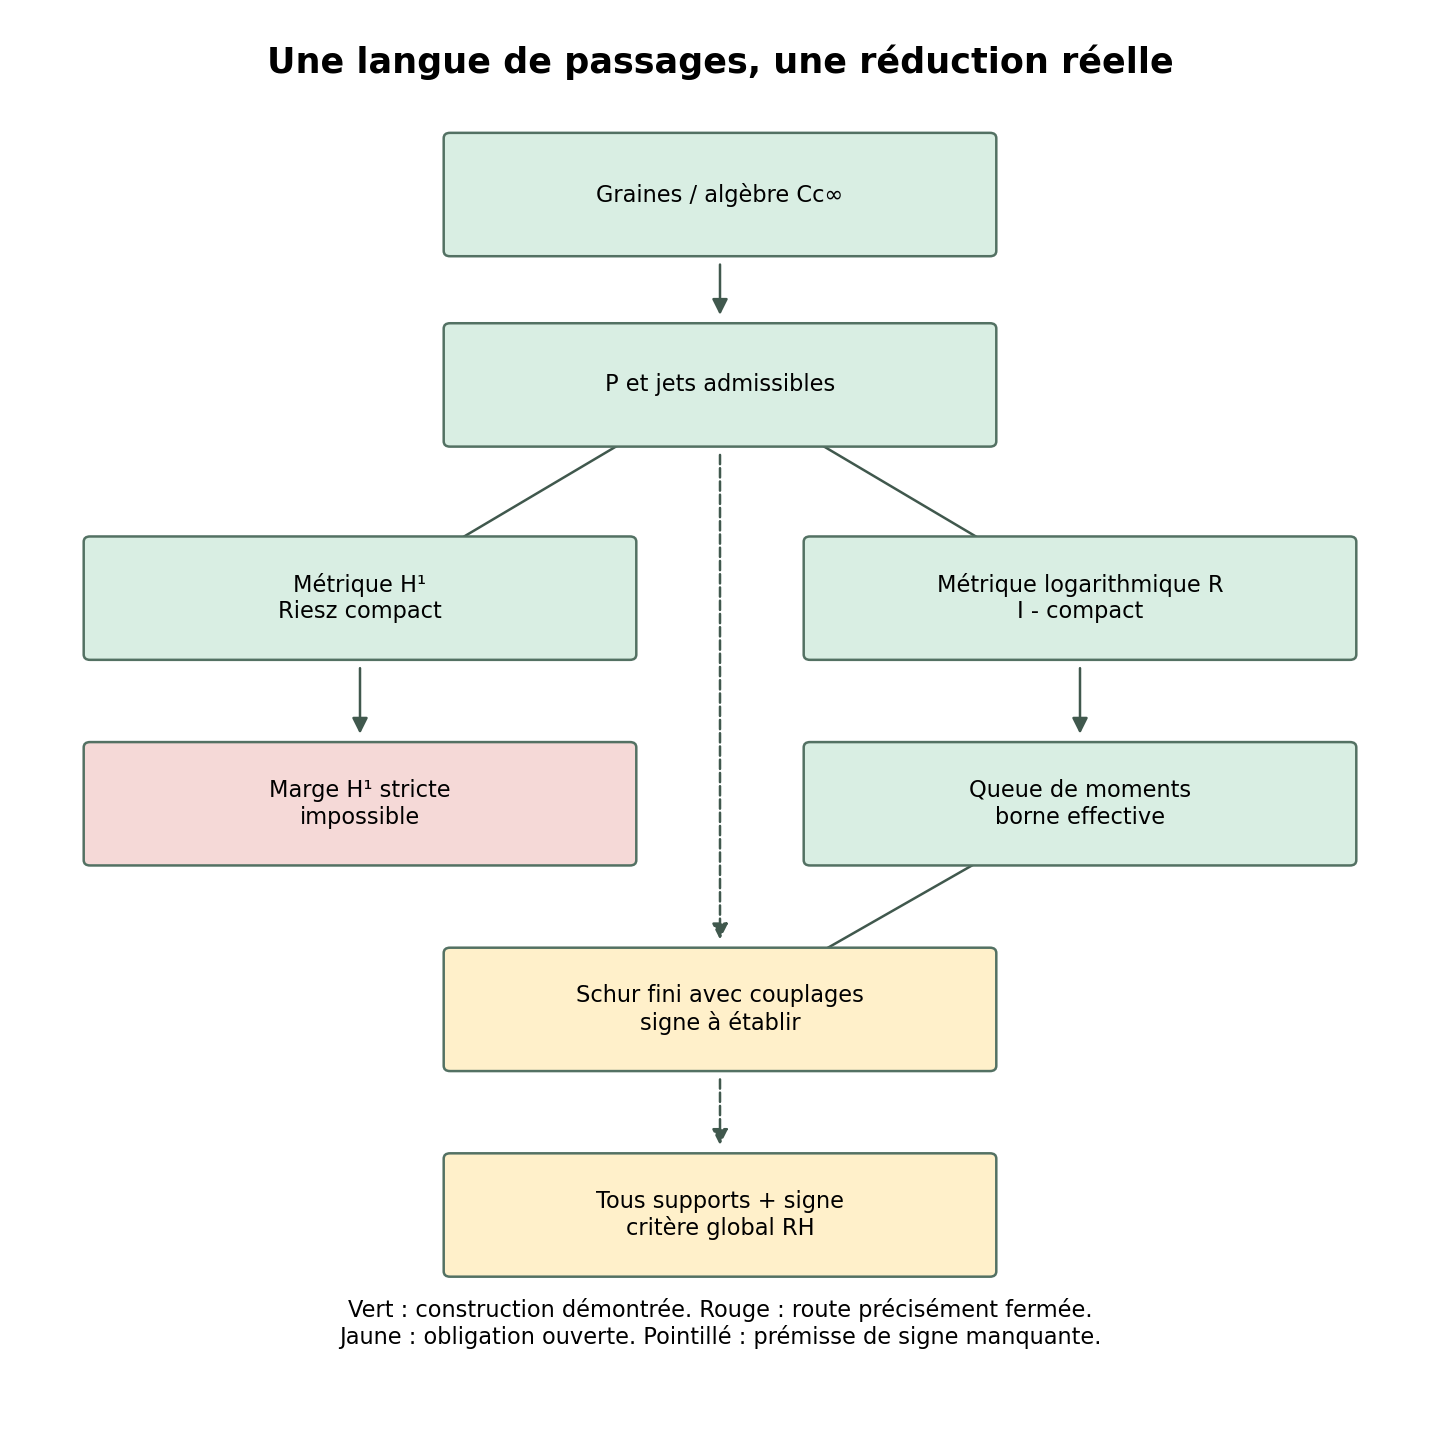
\includegraphics{68_GRAPHE_LANGUE.png}
\caption{Les traductions et leurs obligations.}
\end{figure}

\hypertarget{l1---le-moule-et-sa-muxe9trique}{%
\section{3. L1 - Le moule et sa
métrique}\label{l1---le-moule-et-sa-muxe9trique}}

\textbf{Énoncé.} \(P=D_x^2-1/4:H_0^3(-S,S)\to E_S\) est un isomorphisme.
Pour la norme \(\|\psi\|_{H^3}^2=\sum_{j=0}^3\|\psi^{(j)}\|_2^2\), \[
\|P\psi\|_{H^1}^2=\|\psi'''\|_2^2+\frac32\|\psi''\|_2^2
+\frac9{16}\|\psi'\|_2^2+\frac1{16}\|\psi\|_2^2,
\] \[
\frac1{16}\|\psi\|_{H^3}^2\le\|P\psi\|_{H^1}^2
\le\frac32\|\psi\|_{H^3}^2.
\] \textbf{Preuve.} Deux intégrations par parties donnent
\(\ell_\pm(P\psi)=0\), et les traces de \(P\psi\) sont nulles.
L'expansion des deux carrés \(\|\psi''-\psi/4\|^2\) et
\(\|\psi'''-\psi'/4\|^2\), avec intégration par parties, donne
l'identité. Elle donne injectivité et les bornes indépendantes de S.
Pour \(f\in E_S\), définir \[
\psi(x)=\int_{-S}^x2\sinh((x-y)/2)f(y)\,dy.
\] Alors \(P\psi=f\), \(\psi\in H^3\), et les traces \(\psi,\psi'\)
s'annulent à gauche. Les deux moments les annulent à droite. Comme f a
traces nulles, \(\psi''=f+\psi/4\) s'annule aux deux bords. Ainsi
\(\psi\in H_0^3\). La preuve sur le cœur s'étend par continuité aux
domaines écrits. □

\hypertarget{l2---une-famille-exacte-et-dense}{%
\section{4. L2 - Une famille exacte et
dense}\label{l2---une-famille-exacte-et-dense}}

Poser \[
w_S(x)=(1-x^2/S^2)^4,\quad
\psi_{S,k}=w_S(x)(x/S)^k1_{[-S,S]},\quad f_{S,k}=P\psi_{S,k}.
\] L'annulation d'ordre quatre au bord donne \(\psi_{S,k}\in H_0^4\),
\(\psi_{S,k}\in C^3(\mathbb R)\) et \(f_{S,k}\in H_0^2\subset E_S\). Ces
tests ne sont généralement pas C∞ : leur utilisation repose sur la
continuité H¹ de la forme complète démontrée en V643.

Les graines sont indépendantes, donc les tests le sont par L1. Leur
matrice \(B_{ij}=\langle f_i,f_j\rangle_{H^1}\) est définie positive
exactement. Pour S rationnel, B et les polynômes de corrélation sont
rationnels. Pour \(0\le t\le2S\), \[
h_{ij}(t)=\int_{t-S}^{S}f_i(y)f_j(y-t)\,dy
\] est un polynôme en t, et \(h_{ij}(-t)=h_{ji}(t)\). La corrélation
symétrisée \(H_{ij}=(h_{ij}+h_{ji})/2\) est nulle si i+j est impair. Les
blocs opposés de B et de \(G_W\) sont donc exactement nuls ; les
corrélations croisées individuelles peuvent être non nulles.

\textbf{Densité.} Pour une graine lisse intérieure ψ, le quotient ψ/w\_S
est lisse sur l'intervalle fermé, nul près du bord. Approximer sa
troisième dérivée uniformément par polynômes, puis intégrer trois fois
en fixant les jets à gauche, fournit \(p_n\to\psi/w_S\) dans C³. Donc
\(w_Sp_n\to\psi\) dans H³ et \(P(w_Sp_n)\to P\psi\) dans H¹. Le cœur
admissible dense de V643 et L1 étendent cette approximation à tout E\_S.
□

\hypertarget{l3---invariants-et-relations-conservuxe9es}{%
\section{5. L3 - Invariants et relations
conservées}\label{l3---invariants-et-relations-conservuxe9es}}

Une phase constante et une translation commune conservent h, Q\_W et les
normes invariantes par translation. Les moments se transforment par
\(\ell_\pm(U_af)=e^{\pm a/2}\ell_\pm(f)\). Le support change d'adresse.
La modulation variable \(e^{i\tau x}f\) ne conserve généralement pas les
moments ; moduler une graine avant P produit un autre test admissible.
\[
P(e^{i\tau x}\psi)=e^{i\tau x}(P\psi+2i\tau\psi'-\tau^2\psi).
\] Un changement de support S n'est pas une invariance de la forme.

La traduction multiplicative \(\mathcal L f(u)=u^{-1/2}f(\log u)\) est
unitaire entre les L² correspondants. Sa Mellin vaut
\(M\mathcal Lf(s)=\int f(x)e^{(s-1/2)x}\,dx\). Les deux moments
deviennent les valeurs en 0 et 1 ; les translations deviennent des
dilatations normalisées et des facteurs exponentiels en Mellin.

Une congruence simultanée \((G,B)\mapsto(C^*GC,C^*BC)\), C inversible,
conserve inertie de G et spectre généralisé. Pour un drapeau fixé, les
deux Schur se multiplient par \(|\alpha|^2\) sous
\(v\mapsto\alpha v+w\), w ancien, donc leur quotient est invariant.
Changer de drapeau peut changer les pivots. Si le bloc G est positif
défini, le Schur est un minimum ; s'il est positif singulier, il exige
\(c\in\operatorname{Ran}G\) et G†. Pour un bloc indéfini, la formule
algébrique n'est pas un minimum. □

\hypertarget{l4---une-route-fermuxe9e-dans-huxb9}{%
\section{6. L4 - Une route fermée dans
H¹}\label{l4---une-route-fermuxe9e-dans-huxb9}}

\textbf{Énoncé.} Le Riesz signé de Q\_W sur E\_S muni de H¹ est compact.
Il n'existe aucun \(c>0\) tel que \(Q_W(f)\ge c\|f\|_{H^1}^2\) pour tout
E\_S.

\textbf{Preuve.} Une suite bornée H¹ sur l'intervalle admet une
sous-suite Cauchy L². En dimension un, cela résulte des bornes uniformes
et de \(|f(x)-f(y)|\le\|f'\|_2|x-y|^{1/2}\), puis d'Arzelà--Ascoli. Pour
une différence d bornée H¹ et g de norme H¹≤1, séparer l'intégrale
archimédienne en \((0,r)\) et \((r,\infty)\). La première contribution
est bornée par \(C\int_0^r w(t)t^2dt\to0\), uniformément en g. La
seconde est bornée par \(4\|d\|_2\int_r^\infty w(t)dt\to0\). La masse et
les premiers, en nombre fini, coûtent au plus \(C(S)\|d\|_2\). Ainsi les
images sont Cauchy H¹, ce qui prouve la compactité du Riesz. L'espace
E\_S est infini, par L2. Sur une suite orthonormale e\_n,
\(\|T_Se_n\|_{H^1}\to0\), donc \(Q_W(e_n)\to0\), incompatible avec
c\textgreater0. □

Ce résultat exclut la marge dans cette métrique ; il ne produit aucune
direction négative. Sous positivité, les minima d'une exhaustion dense
tendent vers zéro. Sans positivité, une direction négative peut fixer
une limite négative.

\hypertarget{l5---la-langue-logarithmique}{%
\section{7. L5 - La langue
logarithmique}\label{l5---la-langue-logarithmique}}

Définir une métrique externe \[
R(f)=\|f\|_2^2+\mathcal E(f)
=\int r(\tau)|\widehat f(\tau)|^2d\tau,\qquad r=1+a,
\] \[
a(\tau)=2\sum_{n=0}^\infty\frac{\tau^2}{\beta_n(\beta_n^2+\tau^2)},
\quad\beta_n=2n+\tfrac12.
\] La formule découle de \(w(t)=\sum e^{-\beta_nt}\), Tonelli et
Plancherel. La série converge localement uniformément, car sa queue est
majorée par une constante fois \(\sum\beta_n^{-3}\). Elle est croissante
en \textbar τ\textbar{} et tend vers l'infini par convergence monotone
vers \(\sum2/\beta_n\). Séparer les indices \(\beta_n\le|\tau|\) des
autres donne une croissance de l'ordre logarithmique ; la divergence
suffit aux preuves suivantes.

Le domaine est le Hilbert fermé \[
X_S=\{f:\operatorname{supp}f\subset[-S,S],\ R(f)<\infty,
\ \ell_\pm(f)=0\}.
\] La norme R contrôle L² ; support et moments sont fermés à S fixé. Cet
espace est la complétion logarithmique, avec des fonctions qui ne sont
pas toutes H¹. L'ancien E\_S muni seulement de R n'est pas déclaré
complet.

\textbf{Cœur.} La contraction
\(D_\lambda f(x)=\lambda^{-1/2}f(x/\lambda)\) satisfait
\(r(\tau/\lambda)\le\lambda^{-2}r(\tau)\), pour 0\textless λ≤1, et
converge fortement vers l'identité dans R. Cela se prouve d'abord sur
les transformées Fourier lisses compactes, puis par densité et bornes
uniformes. Elle rentre le support dans l'intervalle. Mollifier avec une
largeur \(\delta<(1-\lambda)S\) conserve ce support intérieur et
converge dans R par domination du multiplicateur Fourier. Les moments,
devenus petits, sont corrigés par deux fonctions fixes φ,φ′ intérieures,
φ paire positive. Leur matrice de moments est inversible ; les
coefficients de correction tendent vers zéro, donc leur coût R aussi. Le
cœur admissible est dense dans X\_S. Comme H¹ se plonge continûment dans
R, L2 donne aussi une famille polynomiale dense dans X\_S. □

\textbf{Compactité.} Sur la boule unité R,
\(\int_{|\tau|>T}|\widehat f|^2\le1/r(T)\). La Fourier restreinte au
rectangle spatial/fréquentiel borné est Hilbert--Schmidt. Les parties
basses fréquences de l'injection \(j_S:X_S\to L^2\) sont donc compactes
et leurs erreurs convergent en norme vers zéro. Ainsi j\_S est compacte.
Avec \[
D_S=(C_0+1)I+\sum_{p^m\le e^{2S}}\frac{\log p}{p^{m/2}}
(U_{m\log p}+U_{-m\log p}),
\] \[
L_S=C_0+1+2\sum_{p^m\le e^{2S}}\frac{\log p}{p^{m/2}},\quad\|D_S\|\le L_S,
\] la même forme s'écrit \[
Q_W(f,g)=R(f,g)-\langle j_Sf,D_Sj_Sg\rangle_2,
\quad T_S^{(R)}=I-C_S,\quad C_S=j_S^*D_Sj_S.
\] C\_S est compact autoadjoint, possiblement signé. Le spectre
essentiel est \{1\}. L'indice négatif et le noyau sont finis à S fixé.
Ce changement de Riesz est un changement de métrique avec domaines
reliés par le cœur, pas une conjugaison unitaire postulée entre H¹ et R.
□

\hypertarget{l6---une-queue-positive-effective}{%
\section{8. L6 - Une queue positive
effective}\label{l6---une-queue-positive-effective}}

Pour \(N\ge0\), définir \[
Y_N=\{f\in X_S:\int x^j f(x)dx=0,\quad0\le j\le N\}.
\] Le reste de Taylor de \(e^{-i\tau x}\), de module au plus
\(|\tau x|^{N+1}/(N+1)!\), et Cauchy--Schwarz donnent \[
|\widehat f(\tau)|^2\le
\frac{S^{2N+3}|\tau|^{2N+2}}{\pi(2N+3)((N+1)!)^2}\|f\|_2^2.
\] En intégrant sur {[}−T,T{]}, \[
\varepsilon_N(T)=\frac{2(ST)^{2N+3}}{\pi(2N+3)^2((N+1)!)^2},\quad
\int_{-T}^{T}|\widehat f|^2\le\varepsilon_N(T)\|f\|_2^2.
\] Si ε\textless1, la partie haute fréquence donne \[
\|f\|_2^2\le\beta R(f),\quad
\beta=\frac1{(1-\varepsilon_N(T))r(T)},\quad
Q_W(f)\ge(1-L_S\beta)R(f)\quad(f\in Y_N).
\] Choisir r(T)\textgreater2L\_S puis ε≤1/2 donne une queue strictement
positive. Les moments ordinaires sont indépendants sur X\_S : si un
polynôme p les annihile, tester \(P\psi\) pour toute graine lisse
intérieure donne \(\int(Pp)\psi=0\), donc Pp=0. Aucun polynôme non nul
ne satisfait cette équation, à cause du terme dominant −p/4. La
codimension est N+1 ; indice négatif plus nullité de la forme sont au
plus N+1. □

\hypertarget{corollaire-entier-calculable}{%
\subsection{Corollaire entier
calculable}\label{corollaire-entier-calculable}}

Soit M le nombre de puissances premières ≤e²ˢ, dont le plafond est
encadré rationnellement dans l'expérience. Les bornes élémentaires
\(C_0+1<8\) et \(\log p/p^{m/2}\le2/e<1\) donnent
\(L_S<\overline L=8+2M\). Poser \[
J=8\overline L,\quad T=2^J,\quad q=\lceil6ST\rceil,\quad N=q-1.
\] Pour n≤T/4, β\_n≤T et chaque terme de a(T) est ≥1/β\_n.~Par
comparaison avec l'intégrale décroissante, \[
a(T)\ge\sum_{n=0}^{T/4}\frac1{2n+1/2}
\ge\frac12\log(T+5)\ge J/4=2\overline L.
\] Nous utilisons \(\log2\ge1/2\). Comme \(q!\ge(q/e)^q\ge(q/3)^q\),
q≥6ST implique \(\varepsilon_{q-1}(T)\le(q/3)4^{-q}\le1/12\le1/2\).
Donc, sans quadrature ni données de zéros, \[
\boxed{Q_W(f)\ge\frac{R(f)}{1+2\overline L}\quad\text{pour }f\in Y_{q-1}.}
\] Ce contrat est effectif et très grossier. La dimension q de la tête
peut avoir des centaines de chiffres : la recette est calculée, la tête
correspondante ne l'est pas. L'enjeu pratique devient de resserrer les
bornes de queue.

\hypertarget{l7---le-schur-fini-garde-linfini}{%
\section{9. L7 - Le Schur fini garde
l'infini}\label{l7---le-schur-fini-garde-linfini}}

Dans \(X_S=F_N\oplus_RY_N\), \(F_N=Y_N^{\perp_R}\), la queue est
représentée par \(A=I-C_Y\) avec \(\|C_Y\|\le\eta=L_S\beta<1\). Son
inverse satisfait \[
\left\|A^{-1}-\sum_{k=0}^mC_Y^k\right\|
\le\frac{\eta^{m+1}}{1-\eta}.
\] Si B est le couplage entre tête et queue, compléter le carré donne
exactement \[
Q_W\ge0\text{ sur }X_S\quad\Longleftrightarrow\quad
G_{\rm eff,S}=G_{FF}-B A^{-1}B^*\ge0.
\] Pour un vecteur v de tête, \(\|b_v\|_R\le L_S\sqrt\beta\|v\|_2\),
donc \[
\langle b_v,A^{-1}b_v\rangle_R
\le\frac{L_S^2\beta}{1-\eta}\|v\|_2^2.
\] La dette calculée par une Neumann tronquée a un reste au plus
\(\eta^{m+1}\|b_v\|_R^2/(1-\eta)\). □

La tête orthogonale est engendrée par les représentants Riesz des
moments. Elle est distincte du préfixe brut des f\_k. Ce dernier fournit
néanmoins un complément direct de Y\_N : sa matrice de moments est le
produit d'une matrice triangulaire de diagonale −1/4 et du Gram monomial
pour le poids w\_S, suivi d'une mise à l'échelle diagonale. Elle est
inversible. Dans ce complément non orthogonal, conserver les couplages
de R est indispensable.

Le théorème de réduction est démontré ; ses prémisses numériques de
calcul effectif restent à fournir : solveur Riesz, projections,
applications de C\_Y, encadrements de leurs erreurs, puis signe de
G\_eff pour tous S.

\hypertarget{l8---arithmuxe9tique-logique-et-symbolique-des-fonctions}{%
\section{10. L8 - Arithmétique, logique et symbolique des
fonctions}\label{l8---arithmuxe9tique-logique-et-symbolique-des-fonctions}}

La langue reçoit une sémantique : \(\mathcal A=C_c^\infty(\mathbb R)\),
algèbre commutative associative de convolution, sans unité parmi les
fonctions. La transformée exponentielle
\(\mathscr Lf(z)=\int e^{zx}f(x)dx\) est entière et traduit la
convolution en produit. Elle devient Mellin sous z=s−1/2, et Fourier sur
z=−iτ à normalisation près.

Les idéaux \[
\mathcal I_r=\{f\in\mathcal A:\partial_z^j\mathscr Lf(\pm1/2)=0,
\ 0\le j<r\},\quad\mathcal I_0=\mathcal A,
\] portent une arithmétique graduée : \[
\mathcal I_r+\mathcal I_s\subset\mathcal I_{\min(r,s)},\quad
\mathcal I_r*\mathcal I_s\subset\mathcal I_{r+s},\quad
\mathcal I_r=P^r\mathcal A.
\] La dernière égalité suit du même inverse compact de P que L1, sur le
cœur lisse, puis de la division du facteur z²−1/4 ; l'ordre d'annulation
baisse d'une unité aux deux points à chaque inverse. Le support inverse
reste dans l'enveloppe convexe, avec possibilité de remplir des trous
intérieurs.

\begin{longtable}[]{@{}lll@{}}
\toprule\noalign{}
Geste & Phrase en transformée & Relation garantie \\
\midrule\noalign{}
\endhead
\bottomrule\noalign{}
\endlastfoot
D\_x f & −z·ℒf & conserve les jets aux ±1/2 ; gagne un ordre en 0 \\
P f & (z²−1/4)·ℒf & gagne un ordre aux ±1/2 ; conserve l'ordre en 0 \\
x f & ∂\_zℒf & perd au plus un ordre à chaque point \\
U\_a f & e\^{}(az)·ℒf & conserve tous les ordres de jets \\
e\^{}(iτx)f & ℒf(z+iτ) & déplace les points d'annulation de −iτ \\
f*g & ℒf·ℒg & additionne les ordres garantis \\
\end{longtable}

Ces identités viennent du changement de variable, de Fubini et de
l'intégration par parties sur des fonctions lisses compactes. Elles
prouvent la correction des règles typées, par induction sur chaque
expression.

La multiplication ordinaire a une autre logique : pour f réel non nul
dans I₁, \(\ell_\pm(f^2)>0\), donc \(f^2\notin I_1\). Convolution et
produit point par point n'ont pas le même contrat. De même,
\(D_x(f*g)=D_xf*g=f*D_xg\) ; D\_x n'est pas une dérivation de
convolution. Le geste position l'est : \(x(f*g)=(xf)*g+f*(xg)\). Pour le
produit ordinaire, \([D_x,x]=I\), et \([P,x]=2D_x\). Les translations
obéissent à \((U_af)*(U_bg)=U_{a+b}(f*g)\) ; une translation commune
n'est pas un automorphisme de cette multiplication. La modulation est un
automorphisme de convolution, mais transporte les idéaux vers d'autres
points.

\hypertarget{les-iduxe9ogrammes-deviennent-une-arithmuxe9tique-de-jets}{%
\subsection{Les idéogrammes deviennent une arithmétique de
jets}\label{les-iduxe9ogrammes-deviennent-une-arithmuxe9tique-de-jets}}

Pour r≥1, les 2r jets normalisés \(\partial_z^j\mathscr Lf(\pm1/2)/j!\)
identifient le quotient \[
\mathcal A/\mathcal I_r\simeq
\mathbb C[\varepsilon]/(\varepsilon^r)\ \oplus\
\mathbb C[\varepsilon]/(\varepsilon^r).
\] Le produit est la convolution de coefficients tronquée, puisque ℒ
transforme * en produit. La surjectivité découle de l'indépendance des
2r fonctionnelles : une relation donnerait
\(e^{x/2}p(x)+e^{-x/2}q(x)=0\), donc p=q=0. Le quotient possède une
unité, même si l'algèbre des fonctions n'en possède pas. Sa codimension
est 2r. Les idéaux descendent strictement, et leur intersection est
\{0\} par analyticité de ℒ et injectivité Fourier.

Une phrase typée est \[
\Gamma\vdash f:\mathcal A(S;r,q;u),
\] avec support dans {[}−S,S{]}, ordres garantis r aux ±1/2 et q en 0,
et unité \(A_{\rm amp}^{u}\). La somme exige mêmes unités et conserve
les minima des ordres ; convolution additionne supports, ordres et
degrés d'unité. P incrémente r, D\_x incrémente q. Ainsi
\(D_x^qP^r\psi\) construit des tests portant ensemble admissibilité
exponentielle et annulations ordinaires de queue. Pour q assez grand
selon L6, cette construction se situe dans une queue positive. Elle ne
couvre pas la tête finie, où le signe reste inconnu.

Trois jets sont distingués : jets du \textbf{test} aux ±1/2 pour
l'admissibilité ; jets du test en 0 pour la queue ; jets d'une fonction
zêta/DH à un zéro critique pour les collisions anciennes. Ils n'ont ni
le même objet ni la même destination. À fenêtre fixée, les conditions
supplémentaires de I\_r, r\textgreater1, ne fournissent pas une
couverture gratuite de tous I₁.

Cette langue est un calcul typé concret, dans des structures existantes
de mathématiques. La création porte sur l'agencement opératoire et
pédagogique. Une nouvelle discipline ou priorité dans la littérature
demanderait un examen bibliographique distinct.

\hypertarget{exuxe9cution-arithmuxe9tique-et-statut-des-valeurs}{%
\section{11. Exécution arithmétique et statut des
valeurs}\label{exuxe9cution-arithmuxe9tique-et-statut-des-valeurs}}

Le protocole \texttt{v644\_protocole\_traductions.json} a été écrit
avant les évaluations : supports 1/2,1,2,3 ; préfixes 2,4,6,8 ;
précisions 40 et 70. L'algèbre des graines, B, corrélations, parité et
plafonds est exacte rationnelle. Poids logarithmiques, intégrales et
spectres sont calculés en multiprécision. Les tableaux ci-dessous sont
générés depuis le journal, sans données de zéros.

\begin{longtable}[]{@{}llll@{}}
\toprule\noalign{}
S & n & minimum généralisé dans H¹ & dette finale normalisée \\
\midrule\noalign{}
\endhead
\bottomrule\noalign{}
\endlastfoot
1/2 & 2 & 1.23247336e-03 & 3.97836799e-03 \\
1/2 & 4 & 3.63960767e-04 & 1.58735551e-03 \\
1/2 & 6 & 3.50380468e-04 & 2.04505554e-03 \\
1/2 & 8 & 2.73158932e-04 & 1.23240641e-03 \\
1 & 2 & 1.04372573e-04 & 2.99224071e-04 \\
1 & 4 & 9.97205293e-07 & 7.24086372e-06 \\
1 & 6 & 1.00483780e-08 & 1.20929786e-04 \\
1 & 8 & 4.50874766e-09 & 1.73657116e-05 \\
2 & 2 & 3.69292367e-06 & 2.75946262e-05 \\
2 & 4 & 2.54223528e-07 & 1.67728557e-06 \\
2 & 6 & 9.60347260e-10 & 2.46022523e-07 \\
2 & 8 & 1.37939583e-11 & 3.98810120e-08 \\
3 & 2 & 1.96709169e-06 & 1.96709169e-06 \\
3 & 4 & 9.68756722e-09 & 1.57818994e-06 \\
3 & 6 & 4.71975518e-11 & 5.77812262e-09 \\
3 & 8 & 5.73023042e-13 & 5.98063018e-10 \\
\end{longtable}

Les 16 minima et les dettes finales sont positifs dans ce diagnostic
numérique. Les deux précisions, les corrélations contre intégration
directe, les deux normalisations archimédiennes, les congruences et le
drapeau recoupent les calculs. Une quadrature multiprécision concordante
n'est pas un intervalle d'erreur validé. Cette expérience ne fournit
donc ni certificat spectral transcendant ni signe global.

\begin{longtable}[]{@{}lllll@{}}
\toprule\noalign{}
S & M & T symbolique & chiffres de q & marge de queue ≥ \\
\midrule\noalign{}
\endhead
\bottomrule\noalign{}
\endlastfoot
1/2 & 1 & 2\^{}80 & 25 & 1/21 \\
1 & 5 & 2\^{}144 & 45 & 1/37 \\
2 & 24 & 2\^{}448 & 136 & 1/113 \\
3 & 98 & 2\^{}1632 & 493 & 1/409 \\
\end{longtable}

Les contrats entiers de queue ci-dessus proviennent d'un corollaire
analytique développé après le pont métrique ; ils ne sont pas présentés
comme une prévision du signe des matrices. Les tailles montrent que
l'existence effective théorique doit encore devenir une méthode de
calcul raisonnable.

\hypertarget{zones-dintuxe9ruxeat-et-prochains-coups-doubles}{%
\section{12. Zones d'intérêt et prochains coups
doubles}\label{zones-dintuxe9ruxeat-et-prochains-coups-doubles}}

\begin{longtable}[]{@{}
  >{\raggedright\arraybackslash}p{(\columnwidth - 6\tabcolsep) * \real{0.2500}}
  >{\raggedright\arraybackslash}p{(\columnwidth - 6\tabcolsep) * \real{0.2500}}
  >{\raggedright\arraybackslash}p{(\columnwidth - 6\tabcolsep) * \real{0.2500}}
  >{\raggedright\arraybackslash}p{(\columnwidth - 6\tabcolsep) * \real{0.2500}}@{}}
\toprule\noalign{}
\begin{minipage}[b]{\linewidth}\raggedright
Zone
\end{minipage} & \begin{minipage}[b]{\linewidth}\raggedright
Contrat acquis
\end{minipage} & \begin{minipage}[b]{\linewidth}\raggedright
Contrat suivant
\end{minipage} & \begin{minipage}[b]{\linewidth}\raggedright
Deux gains attendus
\end{minipage} \\
\midrule\noalign{}
\endhead
\bottomrule\noalign{}
\endlastfoot
Arithmétique des domaines & I\_r=P\^{}r A et jets sous * & moteur
symbolique avec points de jets qualifiés & génération admissible et
invariants auditables \\
Queue logarithmique & ε\_N et marge entière explicites & borne beaucoup
plus fine et validée & taille de tête et marge de queue \\
Schur effectif & inverse et dette bornés & solveur Riesz/projection avec
résidus certifiés & couplages contrôlés et signe fini fiable \\
Loi arithmétique & forme complète et domaines & loi de signe de G\_eff,S
couvrant tous S & interactions premiers/arch et clôture globale \\
\end{longtable}

Bellman pilote des contrats ET/OU : la queue et les couplages doivent se
rejoindre avant une décision de signe. Le coût est déclaré, la
récompense est une obligation effectivement fermée ; aucune probabilité
de RH ni distance arbitraire n'est inventée. Le moteur de V643 demeure
le pilote de scénarios ; la nouvelle grammaire fournit des
transformations à ses actions, sans retoucher ses poids pour forcer un
choix.

Le protocole suivant vise un certificat calculable : choisir S, T et N
avant évaluation ; borner r(T) par sommes positives et reste ; encadrer
ε et L ; construire la tête de moments avec résidus Riesz ; borner la
projection et les actions de C\_Y ; appliquer Neumann avec reste ;
encadrer le Schur effectif. Succès : signe fini avec queue validée pour
le support choisi. Réfutation : direction négative certifiée sous toutes
les gardes. Sinon : indéterminé, avec borne manquante nommée. Une loi
couvrante pour tous les supports constitue une enquête supplémentaire.

Les passages de branches, les collisions doubles et A complexe
arbitraire dans les familles anciennes restent ouverts comme problèmes
propres. Le critère de forme offre une route au signe global qui n'exige
pas de suivre chaque zéro. RH et simplicité des zéros sont également des
buts distincts.

\newpage

\hypertarget{sources-programmes-et-portuxe9e}{%
\section{13. Sources, programmes et
portée}\label{sources-programmes-et-portuxe9e}}

Le lecteur peut vérifier les huit preuves dans ce document et le dossier
local :

\texttt{V644\_LANGUE\_ET\_DOMAINES.md}.

V643, document 67, fournit la normalisation complète, le cœur H¹, le
pont Beurling et Schur singulier. Sources primaires consultées : A.
Beurling, \emph{A closure problem related to the Riemann zeta-function},
PNAS 41 (1955), 312--314, doi:10.1073/pnas.41.5.312 ; A. Connes et C.
Consani, \emph{Weil positivity and trace formula, the archimedean
place}, Selecta Mathematica (2021),
\href{https://alainconnes.org/wp-content/uploads/Selecta.pdf}{texte
auteur}. Leur positivité sous restrictions de support n'est pas
convertie en positivité globale. Weil 1948 est utilisé comme modèle
géométrique documenté en V643 ; sa lecture intégrale et tout transfert
aux entiers restent à établir.

Programmes :

\begin{itemize}
\tightlist
\item
  \texttt{symbolic\_weil\_family.py} : algèbre rationnelle et matrices
  complètes ;
\item
  \texttt{v644\_family\_experiment.py} : exécution prospective ;
\item
  \texttt{v644\_integer\_tail.py} : contrat entier de queue ;
\item
  \texttt{domain\_grammar.py} : calcul de domaines typés.
\end{itemize}

Journaux : matrices, protocole figé, contrats entiers et tests. Les
scripts vérifient l'implémentation de relations représentées ; ils ne
constituent pas une preuve automatisée de RH.

Le document 69 contient le dictionnaire progressif et le registre nommé
complet, plus une grammaire interactive et l'index technique des
fonctions du programme. Les résultats historiques et leurs limites sont
conservés dans le corpus global.

\end{document}
